\documentclass[conference]{IEEEtran}
\IEEEoverridecommandlockouts
% The preceding line is only needed to identify funding in the first footnote. If that is unneeded, please comment it out.
\usepackage{cite}
\usepackage{amsmath,amssymb,amsfonts}
\usepackage{algorithmic}
\usepackage{graphicx}
\usepackage{textcomp}
\usepackage{xcolor}
\usepackage{verbatim}
\usepackage{listings}
% To enable subfigures
\usepackage{caption}
\usepackage{subcaption}
% To prevent URL in bibliographic overflowing to second column
\usepackage[hyphens]{url}

\usepackage{hyperref}

\lstset{
  basicstyle=\ttfamily,
  columns=fullflexible,
  frame=single,
  breaklines=true,
  postbreak=\mbox{\textcolor{red}{$\hookrightarrow$}\space},
  tabsize=4,
}

\graphicspath{ {./images/} }

\lstset{basicstyle=\ttfamily, upquote=true}
\def\BibTeX{{\rm B\kern-.05em{\sc i\kern-.025em b}\kern-.08em
    T\kern-.1667em\lower.7ex\hbox{E}\kern-.125emX}}
\begin{document}

\title{Arbitrary Code Injection in Adblock Plus
% \thanks{Identify applicable funding agency here. If none, delete this.}
}

\author{\IEEEauthorblockN{Eric Li}
\IEEEauthorblockA{Information Networking Institute \\
Carnegie Mellon University\\
Pittsburgh, U.S.A \\
xiaoyili@andrew.cmu.edu}
\and
\IEEEauthorblockN{Teresa Alberto}
\IEEEauthorblockA{
Information Networking Institute \\
Carnegie Mellon University\\
Pittsburgh, U.S.A \\
talberto@andrew.cmu.edu
}
\and
\IEEEauthorblockN{Chengcheng Ding}
\IEEEauthorblockA{
Information Networking Institute \\
Carnegie Mellon University\\
Pittsburgh, U.S.A \\
chengchd@andrew.cmu.edu
}
}

\maketitle

\begin{abstract}
The popularity of extensions that block advertisements is undeniable. Their omnipresence in the browsers of users around the world makes any security vulnerability in these extensions critical. In this article, we will investigate a vulnerability introduced in version 3.2 of Adblock Plus that enabled the execution of arbitrary code on users’ devices, their impact, and what vendors can do to mitigate against it.

We choose Adblock Plus as the adblocking extension to analyze as it is one of the most popular ones with more than tens of millions of downloads on Chrome and Firefox combined. 

Our approach to understanding the vulnerability is, first, to study the full chain of the attack going from the \$rewrite feature implemented in the codebase of Adblock Plus, to the chain of vulnerabilities that can be leveraged by an attacker to gain arbitrary code execution. Based on those insights, we build a proof of concept of the attack, specifying the versions of all of the related software, and providing a skeleton website to demonstrate the attacker's capabilities.

In our experimental setup we reproduce two attack scenarios. First, how an attacker using an open redirect on a victim website, that loads dynamic JavaScript, can abuse the AdBlock Plus \$rewrite rule to force the victim to retrieve malicious JavaScript code. Second, how an attacker using a feature for uploading user content present on a victim’s website, can upload a malicious JavaScript file and force the victim to retrieve it.

For each of these scenarios, we address the mitigations needed to prevent the attack from happening. In the first case, adding connect-src 'self' to CSP defends against this attack. In the second case, CSP doesn’t defend against this attack so we propose as a countermeasure that the victim website cryptographically verify the dynamic JavaScript fetched from the server

% This document is a model and instructions for \LaTeX. This and the IEEEtran.cls file define the components of your paper [title, text, heads, etc.]. *CRITICAL: Do Not Use Symbols, Special Characters, Footnotes, or Math in Paper Title or Abstract.
\end{abstract}

\begin{IEEEkeywords}
browser security, browser extension, ad blocking, XSS
\end{IEEEkeywords}

\section{Introduction}
% Author: Chengcheng Ding
Since the very beginning of their introduction, browser extensions expose additional attack surfaces for browsers. Their popularity among users only makes the matter worse: a vulnerability in a popular extension can affect millions of users. One such popular extension is Adblock Plus, which has tens of millions of users on Chrome and Firefox combined \cite{noauthor_adblockchrome_nodate, noauthor_adblockfirefox_nodate}. In this article, we will investigate a vulnerability introduced in version 3.2 of Adblock Plus that enabled the execution of arbitrary code on users' devices.

The power of Adblock Plus, and any other ad-blocking extension, comes from its filter lists. These lists are composed of a series of URLs with tracking and advertising capabilities, that when visited by the user the extension prevent from loading. Adblock comes with a series of filter lists installed and enabled by default, customized according to the language of the user. In addition, Adblock Plus has a very well-intended feature that allows users to apply custom filter rules. To do so, users can supply a text file that provides (a list of) rule(s) written in the syntax specified by Adblock Plus. Similarly, users can also apply custom filter rules crafted by others to their Adblock Plus extensions. This introduced another party in the threat model.

A standard custom filter rule mentioned above consists of 2 items:
\begin{enumerate}
    \item A pattern of URIs. All requests made to a URI that fits such a pattern will be filtered.
    \item The action to the request that will be filtered. The most obvious and straightforward example would be blocking that request.
\end{enumerate}

In Adblock Plus version 3.2, released on July 17, 2018, a new option for filter action is introduced: rewrite. It allowed users to rewrite requests to a new destination. In that release, it is restricted that the new destination must be of the same origin as the original request. Unfortunately, this introduced new vulnerabilities that allowed arbitrary code execution on user machines that somehow applied malicious filter rules to their extension \cite{abp_code_injection,abp_issue_6622,abp_rewrite_pr,abp_filter_guide}.

We contribute the following:
\begin{enumerate}
    \item An explanation of the technical details behind the attack.
    \item A detailed guide to re-implementing the attack, that specifies corresponding versions of the browser and the extension necessary for the attack to succeed, and a demo website that showcases the attack.
    \item What we can learn from this vulnerability: its impacts, and what vendors can do to mitigate against it.
\end{enumerate}

\section{Background and Goals}
\subsection{Massive Adaptation of Ad-Blocking Extensions}
% Author: Chengcheng Ding
Extensions play a critical role in the capabilities of modern browsers, enabling customized web experiences. Among them is a popular category of extensions that blocks advertisements on web pages. One of the most popular in that category is Adblock Plus. According to statistics from the Chrome extensions web store and Mozilla Firefox add-on store, tens of millions of users have Adblock Plus installed \cite{noauthor_adblockchrome_nodate, noauthor_adblockfirefox_nodate}. According to a study by Pujol et al., 22\% of the most active users analyzed browse the Web with Adblock Plus. In fact, Ad-blocking extensions are so popular that advertisement vendors have begun to take active measures against them \cite{mughees_first_2016}. Therefore, vulnerabilities from the Adblock Plus extension can impact a considerable amount of internet users. That is why we have chosen to investigate a vulnerability in a previous version of Adblock Plus.

\subsection{Adblock Plus business model}
According to Alphabet's financial report, in the last quarter of 2022, the company had a revenue of more than 59,000 million dollars under the category of advertising \cite{alphabet_revenue}. The figures that the online advertising industry manages show why there is a fierce fight between publisher of contents, ad networks and ad-blocking software. Eyeo GmbH business model is not exempt from this dispute. As part of their business model, the company charges fees to big companies to be included in an allow-list as long as the advertisement on their webpages is considered as ``acceptable ads''. This category is defined by an ``acceptable Ads Committee'' created by Adblock's company that counts on the presence of several stakeholders such as Amazon and Dell. The acceptable criteria of an ad depends on its placement on a page, its size and its being distinctive from the main content of the page \cite{acceptable_ads}. Although these commercial deals are not public, the Financial Times published that the fee that Adblock Plus charges to the big companies for being in the whitelist is approximately 30\% of the ad revenues archived by unblocked ads on those sites \cite{financial_times}. 
A caveat related to the links between the stakeholders of the ad industry is that since 2022, the new CEO of Eyeo GmbH is Frank Einecke, a former executive of Google for 14 years.


\subsection{Custom Filters in Adblock Plus}
% Author: Chengcheng Ding
The default advertisement-blocking behaviors of Adblock Plus are defined by a filter list included in the extension. In addition to that, Adblock Plus enables custom filters created by users. These filters allow users to block ads and other unwanted content that may not be covered by the default filter lists. Users can create their own filters by specifying URLs or patterns of URLs, and the actions they want to take against them, such as blocking or allowing. Custom filter lists can also be shared with other Adblock Plus users. From a security standpoint, custom filters involve additional third parties in the flow of ad-blocking, potentially creating additional attack surfaces. The filters are not written in a syntax easily understandable for most average users. Hence, attackers can embed malicious filter actions and present them to users as a filter for additional features, if the filter rules' functionalities allow them.

\subsection{The Rewrite Rule: What and Why}
% Author: Chengcheng Ding
In version 3.2 of Adblock Plus, released on July 17, 2018, a new filter option called ``rewrite'' was introduced. It allows users to rewrite outgoing requests to certain URL(s). In this version, the destination of requests can be rewritten to resources within the same origin. For example, a request to ``foo.com/ad.js'' can be rewritten to ``foo.com/not-ad.js''.

There can be multiple correct usages of the rewrite filter. The first (and primary) one is when simply blocking a request to a certain advertisement-related resource will lead to an error. That's when rewriting the request is a reasonable way to block advertisements with minimal impact on user experience.

Another potential way of using the rewrite filter is eliminating certain HTTP request parameters related to privacy. Advertisers have long used HTTP request parameters for cross-site tracking. Parameters in advertisement links help vendors figure out where the click comes from. Therefore, the rewrite filter can be utilized in this scenario to eliminate request parameters related to tracking.

\subsection{Goals of This Project}
% Author: Chengcheng Ding
There are mainly 2 goals for this project, centered around the vulnerability introduced by the first implementation of the rewrite rule, and its implications.

The first goal is to prove that the vulnerability implies a previously understated attack surface. The vulnerability's chain of exploits utilizes vulnerabilities, or even features, that would be considered low-impact or no-impact on their own. For example, a crucial component of this vulnerability, open redirect, would be considered a feature instead of a vulnerability in many websites. As a matter of fact, Google doesn't consider open redirects to be a security vulnerability to be accepted as part of its Vulnerability Disclosure Program, even while acknowledging it can be a tool for phishers.\cite{noauthor_open_nodate}

The second goal of this project is to recreate a proof of concept of the attack scenario. The proof of concept will specify the versions of all of the related software, and provide a skeleton website to demonstrate the capabilities of the attack. The details of the proof of concept can be found in Section \ref{sec:Implementation}.

\section{Threat model}
The threat model implies a remote attacker with the ability to abuse the rewrite rule of Adblock Plus installed in the victim's browser. There are several possible scenarios for this to happen. First, Adblock Plus is an open-source tool, so a contributor may include a malicious rewrite rule to this open-source codebase being undetected. In addition, the extension comes with several filter rules installed by default, among those is EasyList, a series of filters written by the community. The EasyList file that comes preinstalled with Adblock Plus for English speakers has a total of 58,656 lines, what makes the inclusion of a malicious rule yet more feasible \cite{EasyList}. A second option is an insider threat inside Adblock Plus company to include the malicious rule if enough incentives are offered. Given the number of installations of the extension, an attacker could offer enough economic incentives in exchange of infecting millions of users. A variation of this scenario may happen if a developer of Adblock Plus sees his/her equipment or credentials compromised. In both cases, the attacker needs to include a malicious rewrite rule in the preinstalled filter lists that are enabled by default when installing the extension. 
An alternative scenario would be a malicious actor that convinces the victim to install and enable a malicious filter that includes a malicious rewrite rule in it. Eyeo, the company behind Adblock Plus, makes it clear that the filters are maintained by third parties (even the defaults ones that come preinstalled when installing the extension) and that they neither have control over their contents nor are responsible for any damage provoked to the user in relation to them \cite{abp_suscriptions}.

The victim user needs to have installed a vulnerable version of Adblock Plus in the browser, with the malicious filter enabled. For the attack to succeed the victim needs to visit the page that will be rewritten by the malicious rewrite filter.	

Finally, for the attack to succeed the website that the victim will be visiting needs to fetch resources and load them in the webpage while exposing an open redirect in their website.

\section{Attack Outline}
The attack can be schematized in the fo

\subsection{Victim website}

has an open redirect combined with fetching and loading JS code provokes worse problems.

\subsection{Victim user}

install malicious filter list (may be updated automatically), visit victim website.

\subsection{Attacker}

control the malicious filter list.

\subsection{Potential impact}

\section{Implementation}
\label{sec:Implementation}
% Author: Eric Li

In this section, we explain how we reproduce the attack. We provide a fully functioning environment for demonstrating this attack. We write two websites using Flask as the attacker and the victim website. We also add Content Security Policy (CSP) logics to demonstrate the recommended mitigation in \cite{abp_code_injection}.

To help future researchers reproduce this attack, our project is open source at https://github.com/lxylxy123456/14828. We try to make our work reproducible, such as by providing exact versions of software we use.

\subsection{Recreating the Environment}

As \cite{abp_code_injection} mentions, the rewrite filter vulnerability is only exploitable on Adblock Plus version between 3.2 and 3.5.1. Thus, the first step for us is to find old version of of this extension. Unfortunately, the official Chrome Web Store and Add-ons for Firefox website no longer provide these versions. So we find old versions from unofficial sources.

We are able to find old version of the extension for Chrome on Crx4Chrome \cite{cr4chrome_abp}, a website that provides archived extensions for Chrome. We are unable to find old version of the extension for Firefox easily. However, we argue that since the extension is designed to be browser-independent, the same attack should work on Firefox, Safari, and Edge.

Adblock Plus 3.2 cannot be directly installed on the latest version of Chromium, because the extension is packed in a deprecated format and installing the extension triggers the \lstinline{CRX_HEADER_INVALID} error. However, it is possible to extract the packed extension as a ZIP archive file and install the extension to Chromium in developer mode \cite{stackoverflow_crx_header_invalid}.

The problem with Adblock Plus 3.2 is that it uses manifest V2. However, manifest V2 is deprecated and planned to be removed, so Chromium browsers in the future will not be able to install Adblock Plus 3.2 \cite{chrome_manifest_v2}. Thus, we demonstrate that it is possible to install Adblock Plus 3.2 on an old version of Chromium.

\cite{chromium_old_download} provides guidance to download old versions of the Chromium browser. We choose Chromium 69.0.3497, a version released close to the release date of Adblock Plus 3.2.
Following the guidance, we query the position lookup and find that the branch base position of this version is 576753. Finally, we can download the Chromium browser's snapshot at this version. Adblock Plus 3.2 can be installed directly in Chromium 69, by dragging the CRX package to the browser's extension management page.

In this research, we only test reproducing the attack on Linux. However, since Chromium is a cross-platform browser, we expect the same attack to be reproducible on Windows and macOS.

\subsection{Attacker Website}

We implement the attacker website using Flask as the backend. The host name and port of the attacker website are \lstinline{attacker.local:8080}. We use plain HTML and JavaScript as the frontend. The attacker website has two features.

First, the attacker website hosts an filter rules file that will be loaded to the victim user's browser. To make demonstration easy, we design an interfaces using HTML and JavaScript to modify the filter rules from a browser. The attacker can choose from any subset of the pre-defined 8 rules:

\begin{enumerate}
	\item Block advertisement image.
		% ||*/static/advertisement.png
	\item Block static JavaScript.
		% ||*/static/static.js
	\item Rewrite advertisement image with another image.
		% ||*/static/advertisement.png$rewrite=/static/welcome.png
	\item Rewrite XMLHttpRequest (XHR) that sends private information with URL that does not send private information.
		% ||*/advertisement?city=*&role=*&company=*^$rewrite=/advertisement
	\item Rewrite static Javacsript.
		% ||*/static/static.js$rewrite=/static/static-replace.js
	\item Rewrite dynamic JavaScript to static file.
		% ||*/static/dynamic.js$rewrite=/static/dynamic-replace.js
	\item Rewrite dynamic JavaScript to redirect URL.
		% ||*/static/dynamic.js$rewrite=/redirect
	\item Rewrite dynamic JavaScript to user uploaded file.
		% ||*/static/dynamic.js$rewrite=/upload/user.js
\end{enumerate}

The actual filter: 

\begin{lstlisting}
[Adblock Plus 2.0]
||*/static/advertisement.png
||*/static/static.js
||*/static/advertisement.png$rewrite=/static/welcome.png
||*/advertisement?*^$rewrite=/advertisement
||*/static/static.js$rewrite=/static/static-replace.js
||*/static/dynamic.js$rewrite=/static/dynamic-replace.js
||*/static/dynamic.js$rewrite=/redirect
||*/static/dynamic.js$rewrite=/upload/user.js
\end{lstlisting}

Second, the attacker's website needs to host the malicious JavaScript payload to be executed on the victim's browser. To simplify our design, we host the JavaScript payload statically. The attacker website sets Access-Control-Allow-Origin to \lstinline{"*"} to allow the malicious JavaScript from being read by the victim website on the victim browser.

\subsection{Victim Website}

Similar to the attacker website, we implement the attacker website using Flask as the backend. The hostname and port of the victim website are \lstinline{victim.local:8080}. We use plain HTML and JavaScript as the frontend. The victim website has multiple sections, as discussed below in detail.

\subsubsection{Welcome Image}

The victim website loads a welcome image using HTML's \lstinline{<img>} tag. This provides an image for rewriting the advertisement image later.

\subsubsection{Advertisement Image}

The victim website loads an advertisement image using HTML's \lstinline{<img>} tag. The website also uses JavaScript to detect whether loading the advertisement image is successful. The image is loaded successfully if the \lstinline{load} event listener is called. The image fails to load if the \lstinline{error} event listener is called.

\subsubsection{Targeted Advertisement}

The victim website loads an advertisement using XMLHttpRequest (XHR). The request sends information that undermines the user's privacy, such as the user's location. For demonstration purpose we hard code this information. The server returns an advertisement as a string. The frontend displays the string on HTML.

The purpose of this section is to show that rewrite rules can modify HTTP requests to prevent leakage of users' privacy.

Note that we use XMLHttpRequest (XHR) in the entire demonstration. However, other techniques like fetch also work.

index.html:
\begin{lstlisting}[language=HTML]
<p>
    Targeted advertisement:
    <span id="user_info" class="border">...</span>
</p>
\end{lstlisting}

script.js:
\begin{lstlisting}
{
	const req = new XMLHttpRequest();
	const url = new URL('/advertisement', document.baseURI);
	const params = new URLSearchParams();
	params.set('city', 'pittsburgh');
	params.set('role', 'students');
	params.set('company', 'CMU');
	url.search = params.toString();
	req.addEventListener("load", function() {
		document.getElementById("user_info").innerText = req.responseText;
	});
	req.open("GET", url, true);
	req.send();
}
\end{lstlisting}

\subsubsection{Static JavaScript}

The victim website loads a JavaScript script statically using the \lstinline{<script>} tag in HTML. The loaded script changes HTML to indicate that the script is loaded correctly. This section demonstrates that Adblock Plus is able to block a static script from loading. However, rewrite rules cannot modify the request to load another script instead.

index.html:
\begin{lstlisting}[language=HTML]
<p>
    Static JS:
    <span id="sjs" class="border">...</span>
    <script src="/static/static.js"></script>
</p>
\end{lstlisting}

static.js:
\begin{lstlisting}
document.getElementById("sjs").innerText = "Static JS loaded";
document.getElementById("sjs").className = "success";
\end{lstlisting}

static-replace.js:
\begin{lstlisting}
document.getElementById("sjs").innerText = "REPLACED JS";
document.getElementById("sjs").className = "warn";
\end{lstlisting}

\subsubsection{Dynamic JavaScript}

The victim website loads a JavaScript script dynamically when the user clicks a button. The browser first requests the content of the script using XHR. The browser then evaluates the downloaded script using \lstinline{eval()}. This is similar to how Google Maps dynamically load JavaScripts while the user is browsing the map. Similar to Google Maps, the victim website must enable \lstinline{script-src 'unsafe-eval'} in CSP to make dynamically loading JavaScript working.

index.html:
\begin{lstlisting}[language=HTML]
<p>
    Dynamic JS:
    <span id="djs" class="border">...</span>
    <button id="load">Load</button>
</p>
\end{lstlisting}

dynamic.js:
\begin{lstlisting}
document.getElementById("djs").innerText = "Dynamic JS loaded";
document.getElementById("djs").className = "success";
\end{lstlisting}

dynamic-replace.js:
\begin{lstlisting}
document.getElementById("sjs").innerText = "REPLACED JS";
document.getElementById("sjs").className = "warn";
\end{lstlisting}

\subsubsection{Open Redirect}

One weakness of the victim website is open redirect, where any user can define HTTP redirects in the website \cite{cwe_open_redir}. In the victim website, the attacker can control the URL \lstinline{/redirect} to return an HTTP 302 to any URL. Example URL include a JavaScript on the victim website and a JavaScript on the attacker website.

index.html:
\begin{lstlisting}[language=HTML]
<p>
    Open <a href="/redirect">redirect</a>:
    <input type="name" id="redir_url" value="{{ redir_url }}"
            autocomplete="off"/>
    <br />
    <ul>
        <li class="redir_prefill">/static/dynamic-replace.js</li>
        <li class="redir_prefill">{{ ATTACKER }}/static/exploit.js</li>
        <!-- <li class="redir_prefill">/upload/user.js</li> -->
    </ul>
</p>
\end{lstlisting}

script.js:
\begin{lstlisting}
function send_redir_url() {
	const payload = new FormData();
	payload.append("url", document.getElementById("redir_url").value);
	const req = new XMLHttpRequest();
	req.open("POST", "/redirect");
	req.send(payload);
}

document.getElementById("redir_url").addEventListener("input", send_redir_url);

for (let i of document.getElementsByClassName("redir_prefill")) {
	i.addEventListener("click", function(event) {
		document.getElementById("redir_url").value = this.innerText;
		send_redir_url();
	});
}
\end{lstlisting}

The I'm Feeling Lucky button provided by Google Search has this weakness in 2019. When the user clicks the button, the website sends a GET request to Google's server. The request contains the user's query and \lstinline{btnI} parameter to indicate the user clicks the I'm Feeling Lucky button. Google's server returns an HTTP 302 response to the first Google Search result. An attacker can use this feature as an open redirect. The attacker simply needs to construct a Google Search query that places the redirect target as the first Google Search result. This weakness is fixed by Google later, as discussed in Section~\ref{subsec:google_mitigate}.

\subsubsection{User Uploaded File}

Another weakness of the victim website is user uploaded file with JavaScript content \cite{cwe_upload_file}. The victim website does not perform any sanitization to the file uploaded, and any user of the victim website can view the uploaded file. Thus, if the attacker can trick the victim browser to load the uploaded file, the attacker can achieve arbitrary code execution.

index.html:
\begin{lstlisting}
<p>
    We will host your input at
    <a href="/upload/user.js">/upload/user.js</a>!
    <br />
    <input name="user" id="user" />
</p>
\end{lstlisting}

script.js:
\begin{lstlisting}
document.getElementById("user").addEventListener("input", function(event) {
	const payload = new FormData();
	payload.append("user", this.value);
	const req = new XMLHttpRequest();
	req.open("POST", "/upload/user.js");
	req.send(payload);
});
\end{lstlisting}

\subsubsection{CSP}

The victim website allows dynamically configuring the website's CSP. This allows easy understanding the effectiveness of different defense strategies. In an attempt to defend, the victim user can try to remove \lstinline{script-src *} from CSP and/or to add \lstinline{connect-src 'self'} to the CSP.

index.html:
\begin{lstlisting}
<p>
    CSP: <button id="csp_apply">Apply</button>
    <br />
    
    <input type="checkbox" id="c{{ loop.index0 }}"
        name="c{{ loop.index0 }}" autocomplete="off"
         checked
         class="last">
    <label for="c{{ loop.index0 }}"><tt>{{ line }}</tt></label><br>
    
</p>
\end{lstlisting}

script.js
\begin{lstlisting}
document.getElementById("csp_apply").addEventListener("click", function(event) {
	event.preventDefault();
	location.reload();
});

function handle_check(event) {
	const payload = new FormData();
	for (let i = 0;; i++) {
		const elem = document.getElementById("c" + i);
		payload.append("c" + i, JSON.stringify(elem.checked));
		if (elem.classList.contains("last")) {
			break;
		}
	}

	const req = new XMLHttpRequest();
	req.open("POST", "/csp-list");
	req.send(payload);
}
\end{lstlisting}

\subsection{Attacker User}

The attacker user runs any modern browser that can run JavaScript. The attacker user opens the attacker website and interacts with it. The attacker user also interacts with the victim website by changing the open redirect target and uploading the JavaScript file.

\subsection{Victim User}

We setup the victim user in a Linux virtual machine. The virtual machine runs Chromium 69. We install AdBlock Plus 3.2 and add the filter rules file of the attacker website to AdBlock Plus. The victim user then opens and interacts with victim website. When the attacker updates the filter rules file, the victim needs to click the update button in AdBlock Plus's configuration page.

\subsection{Experiment Results}

Using the setup described above, we perform multiple experiments to demonstrate the capabilities of AdBlock Plus and the arbitrary code execution attack.

\subsubsection{Blocking Image}

AdBlock Plus can block the advertisement image in the victim website. However, the victim website can see that the advertisement image fails to be loaded using the JavaScript \lstinline{error} event listener.

\subsubsection{Blocking Static JavaScript}

AdBlock Plus can block the static JavaScript in the victim website.

\subsubsection{Rewriting Image}

AdBlock Plus can rewrite the advertisement image in the victim website with another image on the victim website. Since the \lstinline{<img>} tag successfully loads an image, the victim website cannot detect the rewrite using the JavaScript \lstinline{error} event listener. This demonstrates that the intended use of the rewrite feature \cite{abp_filter_guide}.

\subsubsection{Rewriting Request Paramters}

AdBlock Plus can rewrite an XHR request to a different URL. In our example, we remove the request URL's query string, which contains private information of the victim user. This is another intended use of the rewrite feature \cite{abp_issue_6622}.

\subsubsection{Rewriting Static JavaScript}

AdBlock Plus is not able to rewrite static JavaScript in the victim website. During the design of the rewrite feature, rewriting static JavaScript is disallowed due to security considerations \cite{abp_issue_6622}.

\subsubsection{Rewriting Dynamic JavaScript}

AdBlock Plus is able to rewrite dynamic JavaScript loaded from XHR request. So when the victim website loads a JavaScript from the its own origin dynamically, AdBlock Plus can change to let it load a different JavaScript from the same origin.

\subsubsection{Attack Using Open Redirect}

A victim website that loads dynamic JavaScript and has the open redirect weakness can be attacked. The attacker first adds AdBlock Plus rule to rewrite the dynamic JavaScript's URL to the open redirect URL. The attacker then controls the open redirect to return HTTP 302 to an attacker-controlled website. The attacker controlled website returns the malicious JavaScript code.

\begin{figure}[htp]
     \centering
     \begin{subfigure}[b]{0.5\textwidth}
         \centering
         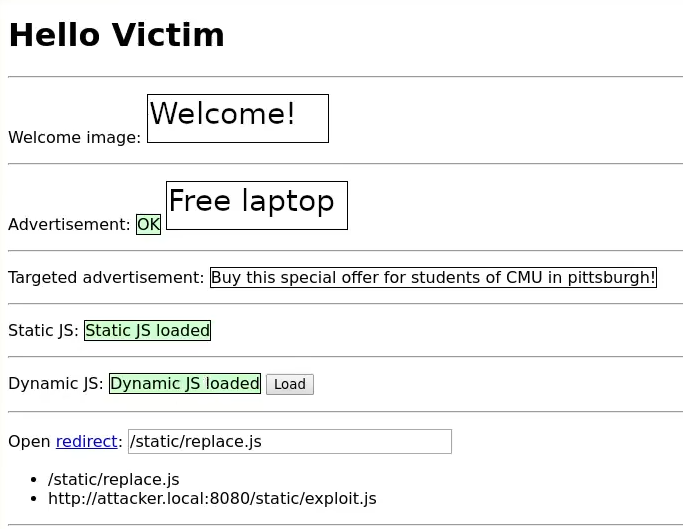
\includegraphics[width=.9\textwidth]{2-figure}
         \caption{Without the malicious filter, the dynamic JavaScript is loaded on the page.}
         \label{fig:non-vulnerable}
     \end{subfigure}
     \hfill
     \begin{subfigure}[b]{0.5\textwidth}
         \centering
         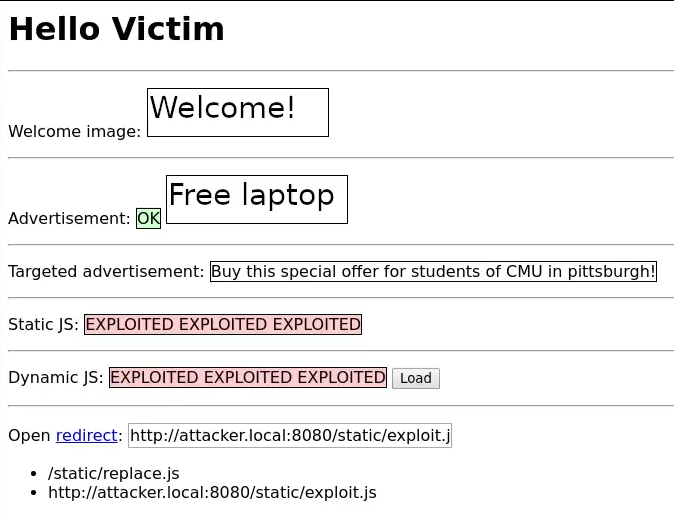
\includegraphics[width=.9\textwidth]{1-figure}
         \caption{With the malicious filter enabled,  AdBlock Plus rewrites the dynamic JavaScript's URL to the open redirect URL, which returns malicious JS code.}
         \label{fig:vulnerable}
     \end{subfigure}
        \caption{Screenshots of a proof of concept website demonstrating the capabilities of the attack.}
        \label{fig:poc}
\end{figure}

Figure \ref{fig:poc} shows a proof of concept website demonstrating in Figure \ref{fig:non-vulnerable} dynamic JS being loaded in a victim's page and in Figure \ref{fig:vulnerable} the same website with the injected attacker's script after the malicious filter is enabled.

Removing \lstinline{script-src *} from CSP does not defend against this attack. The dynamic JavaScript is downloaded using XHR, which is not controlled by \lstinline{script-src}.

Adding \lstinline{connect-src 'self'} to CSP defends against this attack. This rule prevents XHR from being redirected to an origin other than the victim website itself. However, this breaks functionality if the victim website needs to send XHR requests to other websites.

\subsubsection{Attack Using User Uploaded File}

A victim website that loads dynamic JavaScript and has the user uploaded file with JavaScript content weakness can be attacked. The attacker first uploads the malicious JavaScript file to the victim website. The attacker then adds AdBlock Plus rule to rewrite the dynamic JavaScript's URL to the uploaded file.

Neither removing \lstinline{script-src *} from the CSP nor adding \lstinline{connect-src 'self'} to CSP to CSP defends against this attack. The original dynamic JavaScript and the attacker uploaded file are both in the victim website's origin. Thus, blocking loading scripts from the victim website's origin will break the victim website's functionality.

\subsection{Reproducibility Analysis}

To investigate the software versions this attack can take place, we try our experiment in different versions of Chromium and AdBlock Plus.

We see that this attack is successful regardless of the Chromium version, as long as AdBlock Plus can be installed on Chromium. This attack works on both Chromium 69 (released in 2018) and Chromium 112 (released in 2023).

We verify the reproducible AdBlock Plus version range mentioned in \cite{abp_code_injection}. The attack does not work on AdBlock Plus 3.1 (released in May 2018), which does not introduce the rewrite feature yet. This attack works on AdBlock Plus 3.2 (released in July 2018) and 3.5.1 (released in April 2019). We assume this attack works on the versions in between. This attack does not work on AdBlock Plus 3.5.2 (released in April 2019), when the rewrite feature is redesigned to prevent the attack \cite{cr4chrome_abp}.

We also try reproducing this attack on other vulnerable advertisement blockers mentioned in \cite{abp_code_injection}, including AdBlock and uBlock. We are not able to reproduce on uBlock. For unknown reason, uBlock does not recognize any custom filter rules we write.

We are able to reproduce this attack on AdBlock, and the reproducible version range agrees with \cite{abp_code_injection}. The attack does not work on AdBlock 3.31.2 (released in June 2018), which does not introduce the rewrite feature yet. The attack works on AdBlock 3.32.0 (released in July 2018) and 3.44.0 (released in April 2019). We assume this attack works on the versions in between. This vulnerability is fixed in AdBlock 3.46.0 (released in April 2019) \cite{cr4chrome_ab}.

\section{Discussion and Limitations}

\subsection{Warnings During Design Phase}

As Adblock Plus is an open-source project is possible to follow the discussion behind the \$rewrite filter implementation in their issue tracker. Is interesting to note that before this feature was deployed in production several voices raised concerns about the security risks it implied. 
The concerns addressed the risks of a malicious filter author and how platforms with user-uploaded content in the same origin would be endangered \cite{abp_issue_6622}.

As a response, a Software Engineer working for Adblock Plus stated that ``these concerns may represent a risk, a conscious choice we make. One thing we could do is check \$rewrite rules in the known subscriptions (like EasyList) to keep an eye on them'' \cite{abp_issue_6622}.

\subsection{Mitigation by Google}
\label{subsec:google_mitigate}
% Author: Eric Li

When AdBlock Plus 3.2 is published in 2018, Google is vulnerable to this attack because Google Maps loads dynamic JavaScript, and Google's I'm Feeling Lucky provides an open redirect weakness.

Google does not mitigate this attack by removing the dynamic JavaScript. As of April 2023, Google Maps still loads dynamic JavaScript. The CSP of Google Maps contains \lstinline{script-src 'unsafe-eval'}, which is required for calling \lstinline{eval()}.

Google mitigates this attack by removing the open redirect \cite{superuser_ifl_redir_notice}. Google uses the NID cookie to identify different users \cite{google_cookies}. When the user clicks the I'm Feeling Lucky button, Google computes a signature that includes the search query and a secret related to the user. The signature is included in the HTTP request in the \lstinline{iflsig} query field. If the signature verifies, the Google Search server returns HTTP 302 redirect. Otherwise, the server returns an HTML page asking the user to confirm the redirection.

We think this defense is effective. When an attacker constructs the malicious AdBlock Plus rule, he or she cannot compute the signature required for the \lstinline{iflsig} query field. It is possible to compute the signature if the attacker is able to inject cookies to the victim user's browser and overwrites the NID cookie. However, we think this attack is out of scope.

\subsection{Defense by Adblock Plus}
As a mitigation to this security vulnerability, Adblock Plus included a change in its codebase to only allow rewrite redirections to internal resources. These resources are static and included in the source code of the extension. For example ``\$rewrite=abp-resource:blank-js'' makes a redirection to an empty JavaScript. Other internal resources available are an empty blank text (``abp-resource:blank-text''), a blank CSS (``abp-resource:blank-css'') and a transparent gif (``abp-resource:1x1-transparent-gif''), among others. The \$rewrite rule is still present but with a reduced scope, achieving the goal of not only resolving the security concerns of the rewrite but also being able to prevent errors when blocking URLs \cite{abp_filter_guide}. 
    
\subsection{Proposed Mitigation}
% Author: Eric Li

We propose another way for websites to mitigate against this attack, even though the users uses a vulnerable extension like AdBlock Plus 3.2. We mitigate through the process of loading the dynamic JavaScript. Instead of executing whatever string returned in the HTTP response, the victim website should cryptographically verify the dynamic JavaScript fetched from the server.

One possible way to implement asymmetric signatures. The victim server holds a public key and private key pair. When the victim browser loads the victim website, the victim server sends the public key to the victim browser through static JavaScript. When the victim browser requests dynamic JavaScript, the victim server sends the JavaScript content and signs hash of the content using the secret key. The victim browser verifies the signature before calling \lstinline{eval()} on the dynamic JavaScript content.

The disadvantage of this mitigation is that both the server and the browser requires additional computation power and time to compute the cryptographic signature. This will likely increase the delay in the user interaction.

\subsection{Limitations and Future Work}
% Author: Eric Li

In this research, we only investigate the Chromium browser. The main reason is that Chromium browser is popular and old versions of Chrome extensions can be easily downloaded from third-party archives. Though we expect other browsers like Firefox, Safari, and Edge to behave the same, future work is needed to verify this behavior. We expect compiling AdBlock Plus from source when testing on other browsers.

In this research, we also investigate the Linux operating system. Future work is expected to verify whether the attack still works on other operating systems like Windows and macOS.

Since AdBlock Plus 3.2 uses manifest V2, the reproducibility of our demo depends on the browser supporting manifest V2. Chrome is in the process of ending support for manifest V2, but the exact timeline is not determined as of this research \cite{chrome_manifest_v2}. Thus, to reproduce this demo in the future when only manifest V3 is supported, the Chromium browser must be downgraded.

\section{Related Work}
The popularity of extensions and the security risks they impose were addressed in several academic papers \cite{carlini2012evaluation} \cite{barth2010protecting} \cite{bauer2014analyzing}. Carlini et al. \cite{carlini2012evaluation} and Barth et al. \cite{barth2010protecting} focus on a broad security analysis of the Chrome extension ecosystem and its architecture.  In contrast, our research is an insight into the lifecycle of an arbitrary code execution vulnerability in a particular extension.

Similar to our work Bauer et al. paper focuses on attacks of Chrome extensions while implementing proofs of poncepts on each scenario \cite{bauer2014analyzing}. Although their code samples that act as proof of concepts are not publicly available under a Creative Commons License. 

In \cite{10.1145/3433210.3437536} Zafar et al. conduct a thorough study of the privacy implications of Adblock Plus' allow-lists. Although similar to that paper, our research addresses the allow-list (and business model) present on Adblock Plus, our aim is to better explain a threat model for the particular attack addressed. Unlike \cite{10.1145/3433210.3437536} the focus of this paper is guided by a security question and not focused on the privacy implications of Adblock Plus. 

Finally, the research conducted by Alrizah et al. analyzed how Ad-blocking Systems rely on a crowdsourced process to build their filters. The aim of their paper is to analyze the pitfalls of the crowdsourcing process in terms of false positives and false negatives during the blocking of content \cite{10.1145/3355369.3355588}. While \cite{10.1145/3355369.3355588} is not focused on Adblock Plus security vulnerabilities, the study of how the lists are built by third parties in a crowdsourced manner, gives a complementary and useful insight to our work as we mention this fact in terms of the threat model being analyzed.

\section{Conclusion}
% Author: Chengcheng Ding
To conclude this article, we would like to give a review of the vulnerability that allowed arbitrary code execution: The vulnerability is actually composed of multiple low-priority vulnerabilities from different parties. A victim website needs to have open redirect or custom script hosting enabled, which is not even considered a vulnerability for most developers. A victim user needs to apply an Adblock Plus custom filter from another party, which is not expected to lead to an exploit as powerful as arbitrary code injection. Finally, Adblock Plus needs to allow the rewriting of requests to the same origin.
To the parties involved, the corresponding vulnerabilities are most likely considered non-crucial, and will not be prioritized for patching, if patching is considered at all. Unfortunately, all of those little bugs added up to a very formidable exploit. Of course, each party here has good reasons not to prioritize patching those vulnerabilities, as we have studied in the paper. But we believe the major takeaway here is how little vulnerabilities, seemingly innocent on their own, can sum up to a crucial vulnerability, that could potentially affect millions of people. 
\section*{Acknowledgment}
We would like to thank Hanan Hibshi for her insightful comments throughout the course of our research, and for having shown us a prolific field of study in the area of security such as browser extensions. This paper is a final project for the course ``Browser Security'' of the Master of Science in Information Technology-Information Security (MSIT-IS) and Master of Science in Information Security (MSIS) postgraduate programs at Carnegie Mellon University. 

We would like to dedicate a special thanks to our peers who during the course provided us with feedback to improve the project.

\bibliographystyle{IEEEtran}
\bibliography{references}

\begin{appendices}

\section{Peer reviews we have received}

\begin{enumerate}
    \item In the demo when the dynamic javascript is rewritten, the static javascript is also rewritten. If possible, we think separating those scripts in the demo may gave the audience a clearer understanding.
    \item In the ``IMPLEMENTATION'' section of the draft, it was mentioned that ``Adblock Plus version between 3.2 and 3.5.1'', yet, the ``reproducibility analysis'' section mentions that ``This attack works on AdBlock Plus 3.2 (released in July 2018) and 3.5.1 (released in April 2019)''. We think that rephrasing the later sentence to ``This attack works on version between AdBlock Plus 3.2 (released in July 2018) and 3.5.1 (released in April 2019)'' might be clearer than before.
    \item As mentioned in the first slides of the final presentation, the business model of Eyeo GmbH is an interesting model. We think it would be worth mentioning about how the business model affects Ablock Plus's usability from a user's perspective.
    \item To our knowledge, the Brave Browser has its own engine for Adblock named AdBlock-rust and it supports Adblock Plus syntax. Is there a possibility that past version of Adblock-rust would also be vulnerable?
    \item On the browser side, Adblock Plus does maintain a version for Microsoft Edge. Would Edge also be vulnerable for the same version of Adblock Plus?
\end{enumerate}

\section{Respond to peer review}

This section records our responses to the peer review.

% Author: Eric Li
The first comment is about the replace script changing both static JS and dynamic JS's HTML elements, which creates confusion. As a response, we modify the demo to only change one of static JS and dynamic JS.

% Author: Eric Li
The second comment is about Section \ref{sec:Implementation} mentioning only the start and end version of vulnerable extensions, without mentioning the versions in between. The peer reviewer suggests changing the sentences to ``between version X and Y.'' However, we choose to keep our writing because we want to only report what we tested. We add a sentence to state that the versions in between are assumed to be reproducible, though we did not test them.

The third comment is about the business model of Adblock Plus and how it affects the usability of the extension from a user's perspective. A usability analysis was not included in our analysis as we focus on the technical security aspects of the vulnerability present in the extension. As a threat from inside the company was a possible scenario in the threat model, it seems pertinent to understand the business model of the company that owns Adblock. Nevertheless, a usability evaluation of the extension is out of the scope of the research.

% Author: Eric Li
The fourth comment is about the Brave browser. We consider the Brave browser as out of scope. Through superficial research on its code base, it seems this browser implements advertisement blocking logic through Rust, which is different from AdBlock Plus. The advertisement blocking code does not contain the keyword ``rewrite'' in the context of the rewrite feature discussed in this paper, so we think Brave browser is not vulnerable.

% Author: Eric Li
The fifth comment is about Microsoft Edge. In our older draft of the paper we only mention Chrome (Chromium), Firefox, and Safari. We modify the paper to add Edge, since Edge is also a popular browser. We still assume the attack works on Edge with out actually testing, because as far as we know, Edge only works on Windows, but we are testing on Linux.

\end{appendices}
\end{document}

\begin{table}[htbp]
\caption{Table Type Styles}
\begin{center}
\begin{tabular}{|c|c|c|c|}
\hline
\textbf{Table}&\multicolumn{3}{|c|}{\textbf{Table Column Head}} \\
\cline{2-4} 
\textbf{Head} & \textbf{\textit{Table column subhead}}& \textbf{\textit{Subhead}}& \textbf{\textit{Subhead}} \\
\hline
copy& More table copy$^{\mathrm{a}}$& &  \\
\hline
\multicolumn{4}{l}{$^{\mathrm{a}}$Sample of a Table footnote.}
\end{tabular}
\label{tab1}
\end{center}
\end{table}

\begin{figure}[htbp]
\centerline{
\includegraphics{fig1.png}}
\caption{Example of a figure caption.}
\label{fig}
\end{figure}

